\documentclass[landscape]{standalone}
\usepackage{tikz}
\usetikzlibrary{automata}
\begin{document}
\begin{center}
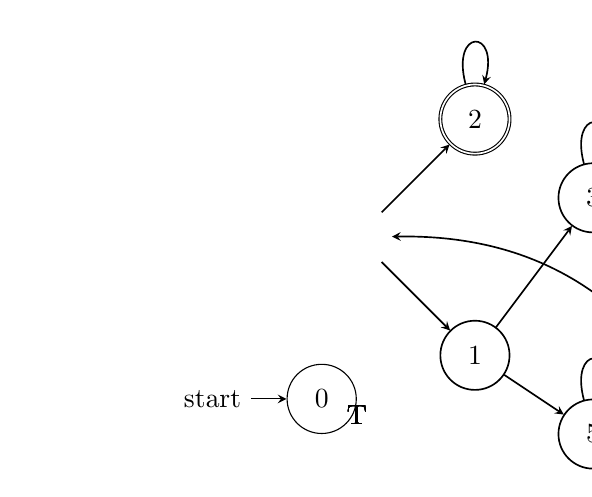
\begin{tikzpicture}[->,>=stealth,auto,node distance=2.5cm,semithick]
\tikz [every edge quotes/.style={fill=white,font=\footnotesize}]
\node[state, initial] (0) at (0.0,2.5) {0};
\node[state] (1) at (1.5,1.0) {1};
\node[state, accepting] (2) at (1.5,4.0) {2};
\node[state] (3) at (3.0,2.9999999999999813) {3};
\node[state] (4) at (4.5,2.9999999999999813) {4};
\node[state] (5) at (3.0,-1.84297022087776e-14) {5};
\node[state] (6) at (4.5,-1.8540724511240114e-14) {6};
\path (0) edge[->] (1) node[pos=0.5, above] {T};
\path (0) edge[->] (2) node[pos=0.5, above] {T};
\path (1) edge[->] (3) node[pos=0.5, above] {T};
\path (1) edge[->] (5) node[pos=0.5, above] {T};
\path (3) edge[->] (4) node[pos=0.5, above] {T};
\path (4) edge[->] (3) node[pos=0.5, above] {T};
\path (5) edge[->] (6) node[pos=0.5, above] {T};
\path (6) edge[->, bend right] (0) node[pos=0.5, above] {T};
\draw[->, loop above] (2) to (2);
\draw[->, loop above] (3) to (3);
\draw[->, loop above] (5) to (5);
\end{tikzpicture}
\end{center}
\end{document}